\section{Project description and critical review}

\subsection{Problem framing and research aim}

The approved project asks how three battery-limited drones can repeatedly inspect known, changing wildfire hazards over a finite mission. The controller must trade inspection freshness against transit energy, overdue locations, scarce charging capacity and collision restrictions. This is not a hidden-fire discovery experiment: fire, fuel, terrain, priority, wind and drone condition are fully observed in the simulation \cite{source1}, \cite{source12}. Novelty is a coordinated sequential decision problem, not the claim that deep RL necessarily wins against engineered patrol rules. Related peer-reviewed drone-fire studies justify the application domain but do not calibrate the parameters of this simulator \cite{source9}, \cite{source10}.

Why nontrivial: an action that increases coverage now can strand a drone later; high-priority sites change with burning cells and fire front; three simultaneous moves can interfere; and all drones share one charger. A one-step urgency rule may nonetheless be formidable. The suitable scientific question is whether learned policies yield measurable sustained inspection improvement under an unchanged task and comparable held-out scenarios.

\subsection{Fully observable finite-horizon MDP}

Decision process: M=(S,A,P,r,$\gamma$,H). The observation is a Gymnasium dictionary: five full-grid maps---burning, normalized fuel, terrain susceptibility, static priority, and inspection age---of shape (5,n,n); three records {[}row,column,battery,lost{]} of shape (3,4); and 12 global entries for wind (five one-hot categories), charger ownership (four), base coordinates (two), and remaining-time proportion (one). In the main study n=40 and H=300. Each variable is normalized to {[}0,1{]}. The neural encoder additionally constructs four binary location maps from these observed coordinates, yielding nine spatial channels and 24 nonspatial inputs. It does not supply hidden future fire information \cite{source12}, \cite{source13}.

One central action controls all three drones. Each receives one of stay/north/south/west/east; the joint discrete space therefore has 5$^3$=125 actions. Inspection happens automatically after movement. At the shared base, a staying drone can charge, but only one charger owner is serviced per step. A physical transition resolves simultaneous moves and blocked collisions, applies energy and charge updates, increments and resets inspection ages, computes reward, then evolves fire and wind. Full fleet loss or the horizon ends an episode. Transition randomness is seeded; parameters are illustrative rather than physically calibrated \cite{source12}.

The 40$\times$40 environment uses battery capacity 160, movement cost 1, hover cost 0.25, recharge rate 8, radius 2, inspection deadline 30, initial three fires, base near the grid centre, fire-spread probability 0.04 and wind-change probability 0.06. Three higher-priority zones are initialized per scenario. Terrain influences fire, not obstacles to flight. The single controller cannot be equated with three independent learning agents.

\subsection{Objective, reward and measurable outcomes}

The simulator computes location priority w\_i = p\_i(1 + 2 b\_i + f\_i), where p\_i is static site priority, b\_i marks burning cells and f\_i marks a fuel-bearing fire-front neighbour. At each step, weighted freshness is F\_t = $\sum$\_i w\_i max(0,1-age\_i/deadline) / $\sum$\_i w\_i. The overdue fraction is the weighted proportion with age\_i \textgreater{} deadline. These are quality metrics on a {[}0,1{]} scale, not the percentage of area covered \cite{source12}.

The environment reward is the sum of weighted inspection gain, a negative overdue penalty, normalized energy cost, blocked collision attempts and newly lost drones, plus a remaining-horizon overdue charge on total fleet failure. Frozen weights are +1.0 gain, -0.1 overdue fraction, -0.02 $\times$ energy/160, -0.2 per blocked command and -5 per new drone loss. This reward is shaped in the general sense of combining terms, but the main 40$\times$40 experiment sets additional coordination shaping to zero. Distinguish this existing multi-term objective from a proposed potential-based shaping method \cite{source8}.

Report distinct metrics: full-horizon weighted freshness, overdue fraction, episode return, energy, loss count, collision attempts, fleet-failure rate, charge completions and safe-return events. A safe return event is not an assertion that all drones ended at base. On an early total fleet failure the evaluator pads unserved timesteps with zero freshness and fully overdue locations rather than rewarding a shortened run \cite{source1}, \cite{source12}.

\subsection{Selection and implementation of three RL methods}

DQN (value-based): a convolutional encoder maps the full observation to 125 joint Q-values; replay samples transitions; a target network supplies bootstrapped TD estimates; epsilon-greedy data collection explores admissible candidate actions. The final corrected masked DQN uses a feasible next-action TD maximum and standard DQN targets, not Double DQN \cite{source2}, \cite{source13}.

REINFORCE (Monte Carlo policy gradient): a categorical policy over feasible joint actions collects full episodes, then weights log-probabilities by discounted reward-to-go minus an optional learned Monte Carlo baseline. It contains no TD bootstrap, despite sharing the neural encoder with the other methods \cite{source3}, \cite{source13}.

A2C (synchronous actor--critic): one network returns categorical policy logits and a state-value estimate; 32-step rollouts use bootstrapped discounted targets to update policy and critic. Its entropy penalty regularizes action selection; it is synchronous single-environment A2C, not the asynchronous A3C algorithm described by Mnih et al. \cite{source4}, \cite{source13}.

Algorithm--code mapping to independently validate: environment reset/step in src/wild\_drone/environment.py; action\_mask and masked TD target in masked\_learning.py; neural encoder, return and TD utilities in learning.py; candidate and Greedy/sweep policies in baselines.py; experiment runner, audit and replay scripts in scripts/. The consolidated Wildfire\_Drone\_Fleet.ipynb already provides implementation-oriented pseudocode; students must verify and attribute each assessed code/notebook section.

\subsection{Experiments and training decisions}

Historical development used 20$\times$20 worlds to diagnose poor unmasked survival, repeated commands, instability and incomplete charger coordination. Changes included spatial drone/base channels, REINFORCE's Monte Carlo baseline, feasible-action rules, lower DQN learning rate, Double DQN screening and diagnostic supervised probes. These experiments must not be merged with the final 40$\times$40 numerical estimates or described as successful RL tuning without evidence \cite{source1}, \cite{source14}, \cite{source15}.

The frozen main comparison used independently initialized training seeds 0, 1, 2 for each of DQN, REINFORCE and A2C (nine fits). Each completed 300 episodes on training worlds 0--299 (90,000 environment interactions per fit, 810,000 total). All final checkpoints were evaluated on unseen worlds 22000--22019: 9$\times$20=180 learned-policy missions plus 4$\times$20=80 baselines, totalling 260. No 40$\times$40 best-checkpoint selection, post-result tuning, supervised warm start or additional coordination shaping was used \cite{source1}, \cite{source11}.

Shared settings include $\gamma$=0.99, Adam, gradient clipping 0.5 and a common spatial input. DQN: learning rate 1$\times$10$^{-}$$^4$, minibatch 32, replay capacity 2,000, target refresh every 100 update steps and epsilon 1$\rightarrow$0.05 over 40,000 steps. REINFORCE: learning rate 1$\times$10$^{-}$$^3$ and entropy weight 0, with a learned Monte Carlo baseline. A2C: learning rate 1$\times$10$^{-}$$^4$, 32-step rollout and entropy weight 0.05. These are fixed study choices, not proof of optimum settings \cite{source11}.

\subsection{Frozen 40$\times$40 outcomes}

\begin{table*}[!t]
\centering
\caption{Audited main-study evaluation means across 260 missions.}
\scriptsize
\setlength{\tabcolsep}{4pt}
\begin{tabular}{lrrrr}
\toprule
\textbf{Policy} & \textbf{Fresh. $\uparrow$} & \textbf{Overdue $\downarrow$} & \textbf{Return $\uparrow$} & \textbf{Loss $\downarrow$} \\
\midrule
DQN & 0.08438 & 0.86869 & -24.79 & 0 \\
REINFORCE & 0.06901 & 0.89402 & -25.81 & 0 \\
A2C & 0.08435 & 0.86949 & -24.83 & 0 \\
Greedy & 0.22077 & 0.65563 & -16.10 & 0 \\
Sweep & 0.06486 & 0.90121 & -26.07 & 0 \\
Random & 0.05956 & 0.92098 & -42.87 & 3 \\
Masked random & 0.08379 & 0.88601 & -25.46 & 0 \\
\bottomrule
\end{tabular}
\end{table*}

\begin{figure}[!t]
\centering
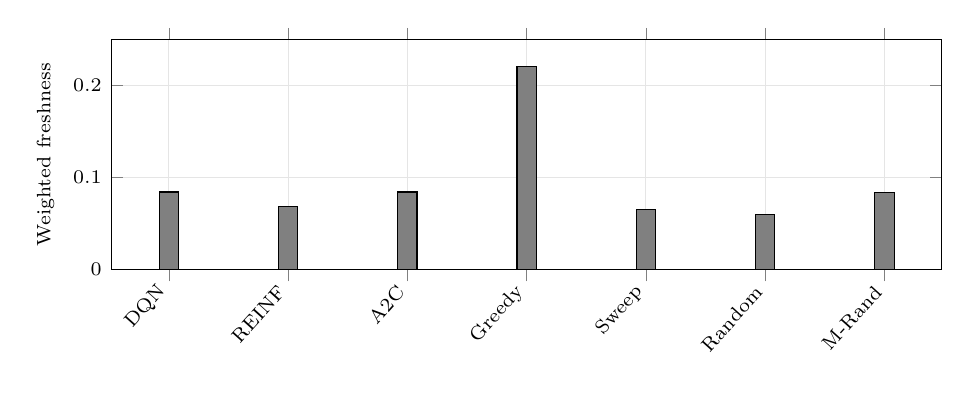
\begin{tikzpicture}
\begin{axis}[ybar,width=\columnwidth,height=4.5cm,bar width=7pt,ymin=0,ymax=.25,ylabel={Weighted freshness},symbolic x coords={DQN,REINF,A2C,Greedy,Sweep,Random,M-Rand},xtick=data,x tick label style={rotate=48,anchor=east,font=\scriptsize},ylabel style={font=\scriptsize},yticklabel style={font=\scriptsize},grid=major,major grid style={gray!20},enlarge x limits=.08]
\addplot[fill=black!50,draw=black] coordinates {(DQN,.08438) (REINF,.06901) (A2C,.08435) (Greedy,.22077) (Sweep,.06486) (Random,.05956) (M-Rand,.08379)};
\end{axis}\end{tikzpicture}

\caption{Main-study freshness means; illustrative graph redrawn from published study statistics \cite{source1}.}
\end{figure}

The Greedy policy has approximately 2.62$\times$ DQN's mean freshness and 3.20$\times$ REINFORCE's. DQN improves over masked random by only 0.000589 freshness (0.059 percentage points); A2C by 0.000553; REINFORCE is below it by 0.014780. All learned methods miss the prespecified all-seed contribution and Greedy capability gates. An intact fleet at the horizon did not imply good monitoring. Unmasked random loses all three drones in each of its 20 test missions, whereas all nine masked fitted policies and masked random have zero average losses \cite{source1}.

Statistical caution: each learned controller's average first aggregates 20 worlds within each fitted seed, then averages three seed means. Freshness seed-level sample SD is DQN 0.00254, REINFORCE 0.00730 and A2C 0.01163. Baseline variability is across 20 worlds, a different unit. Three fitted replicates are insufficient for strong significance or convergence claims. DQN's +0.000589 average difference is descriptive, not evidence of a meaningful positive effect \cite{source1}.

\begin{figure}[!t]
\centering
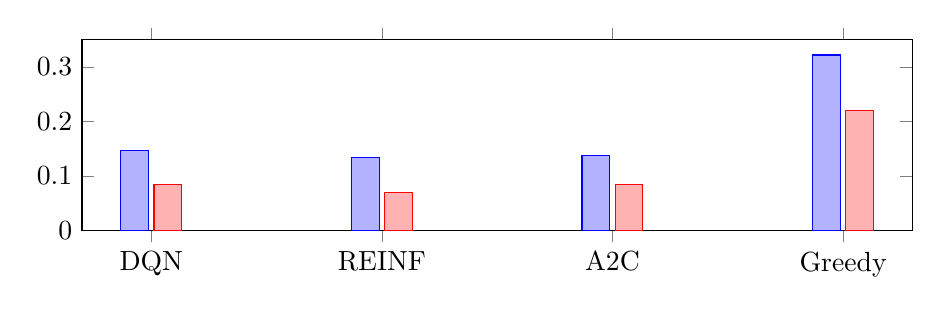
\begin{tikzpicture}
\begin{axis}[ybar,width=\columnwidth,height=4cm,ymin=0,ymax=0.35,symbolic x coords={DQN,REINF,A2C,Greedy},xtick=data]
\addplot coordinates {(DQN,.14585) (REINF,.13343) (A2C,.13694) (Greedy,.32203)};
\addplot coordinates {(DQN,.08438) (REINF,.06901) (A2C,.08435) (Greedy,.22077)};
\end{axis}
\end{tikzpicture}

\caption{The 20$\times$20 and 40$\times$40 values come from different code/configuration regimes; do not infer an isolated scaling effect \cite{source14}.}
\end{figure}

\subsection{Critical review: separating task completion from RL success}

The implementation and audit objectives were substantially met: an explicit MDP, independently implemented three-method comparison, notebook-linked pseudocode, multiple historical pilots, fresh-world evaluation, and a completed 40$\times$40 training protocol. Independent replay checked all 75,911 final evaluation steps, selected actions, masks, state hashes and rewards, with zero neural-score drift. This supports reproducibility of the recorded experiment, not validation of real wildfire physics \cite{source1}, \cite{source11}.

The central scientific finding is negative. DQN and A2C lie close to a policy that uniformly samples rule-approved actions; REINFORCE performs worse. Feasible-action filtering blocks unsafe battery/collision commands and is a dominant explanation for survival. Because Greedy uses its native candidate logic and supervised probes have separate objectives, the comparison is not a perfectly identical algorithmic control. The absence of validated learning superiority must be stated plainly \cite{source1}, \cite{source14}.

Potential mechanisms supported by historical diagnostics include a large 125-way joint action head, difficult long-horizon inspection/charging credit assignment, weak learned ranking under distribution shift, repeated argmax actions and (in earlier unmasked 20$\times$20 runs) very large Q predictions relative to bounded return. The 40$\times$40 audited experiment does not identify one unique causal mechanism. Earlier pilot changes were not isolated one-factor causal estimates, and additional compute alone does not resolve why a Greedy controller wins \cite{source14}, \cite{source15}.

Construct validity is limited: true fire and wind are observed; the grid ignores smoke occlusion, uncertain sensors, no-fly zones and calibrated physical units; fire evolves through synthetic stochastic cellular rules. External validity to actual UAV emergency operations has not been established. Also, the 20$\times$20 and 40$\times$40 comparison changes horizons, energy settings, sensor radius, inspection deadline and source revision, so the observed numerical difference is not a controlled scalability result \cite{source12}, \cite{source14}.
